% Crucial Preamble
\documentclass[12pt,letterpaper]{article} \usepackage{amsmath} \usepackage{graphicx} \usepackage[margin=1in]{geometry} \usepackage{longtable}  \usepackage{amssymb}

% Extra Preamble
\usepackage{fancyhdr} \usepackage{enumitem} \usepackage{float} \usepackage{soul}
\usepackage{multicol} \usepackage[compact]{titlesec}


% frames with display breaks
\usepackage{mdframed}
\allowdisplaybreaks

% change spacing
\usepackage{setspace}
\setlength{\parskip}{0.4\baselineskip}

% Remove paragraph indentation
\setlength{\parindent}{0pt}

% Reduce space before and after section headings
%\titlespacing*{\section}{0pt}{0.1\baselineskip}{0.2\baselineskip}

% changes font
%\renewcommand{\familydefault}{\sfdefault}

% adds header and footer
\pagestyle{fancy}
\fancyhead{} \fancyhead[C]{ELG 3125 Summary Sheet} \fancyhead[L]{ELG3125} \fancyhead[R]{Owen Daigle}
\fancyfoot{} \fancyfoot[C]{\thepage}


\begin{document}
	
	\begin{center}
		\Large\textbf{ELG 3125 Summary Sheet} \\
		\vspace{0.5em}
	\end{center}	

	\section{Basics of Signals and Systems}
	We can have a signal that is either continuous or discrete. These signals are represented as math functions.
	\begin{figure}[!h]
		\centering
		\includegraphics[width=0.8\linewidth]{"images/discrete vs cont"}
		\label{fig:discrete-vs-cont}
	\end{figure}
	Computers always will display and work with a discrete signal. However often it is to model a continuous signal. 
	
	We call a signal a power signal if its average power is finite. Similarly, we call a signal an energy signal if its total energy is finite. 
	
	\begin{mdframed}
		\textbf{Ex. } A 120VAC wall outlet is a power signal.
		
		This is because the average power is finite. If we have for example a 1500w heater connected, it will always draw 1500W. 
		
		However if we keep it running for a long time, it will use a very large amount of energy. So it is infinite energy.
	\end{mdframed} 
	
	\subsection{Transformations}
	There are many transformations.
	\begin{figure}
		\centering
		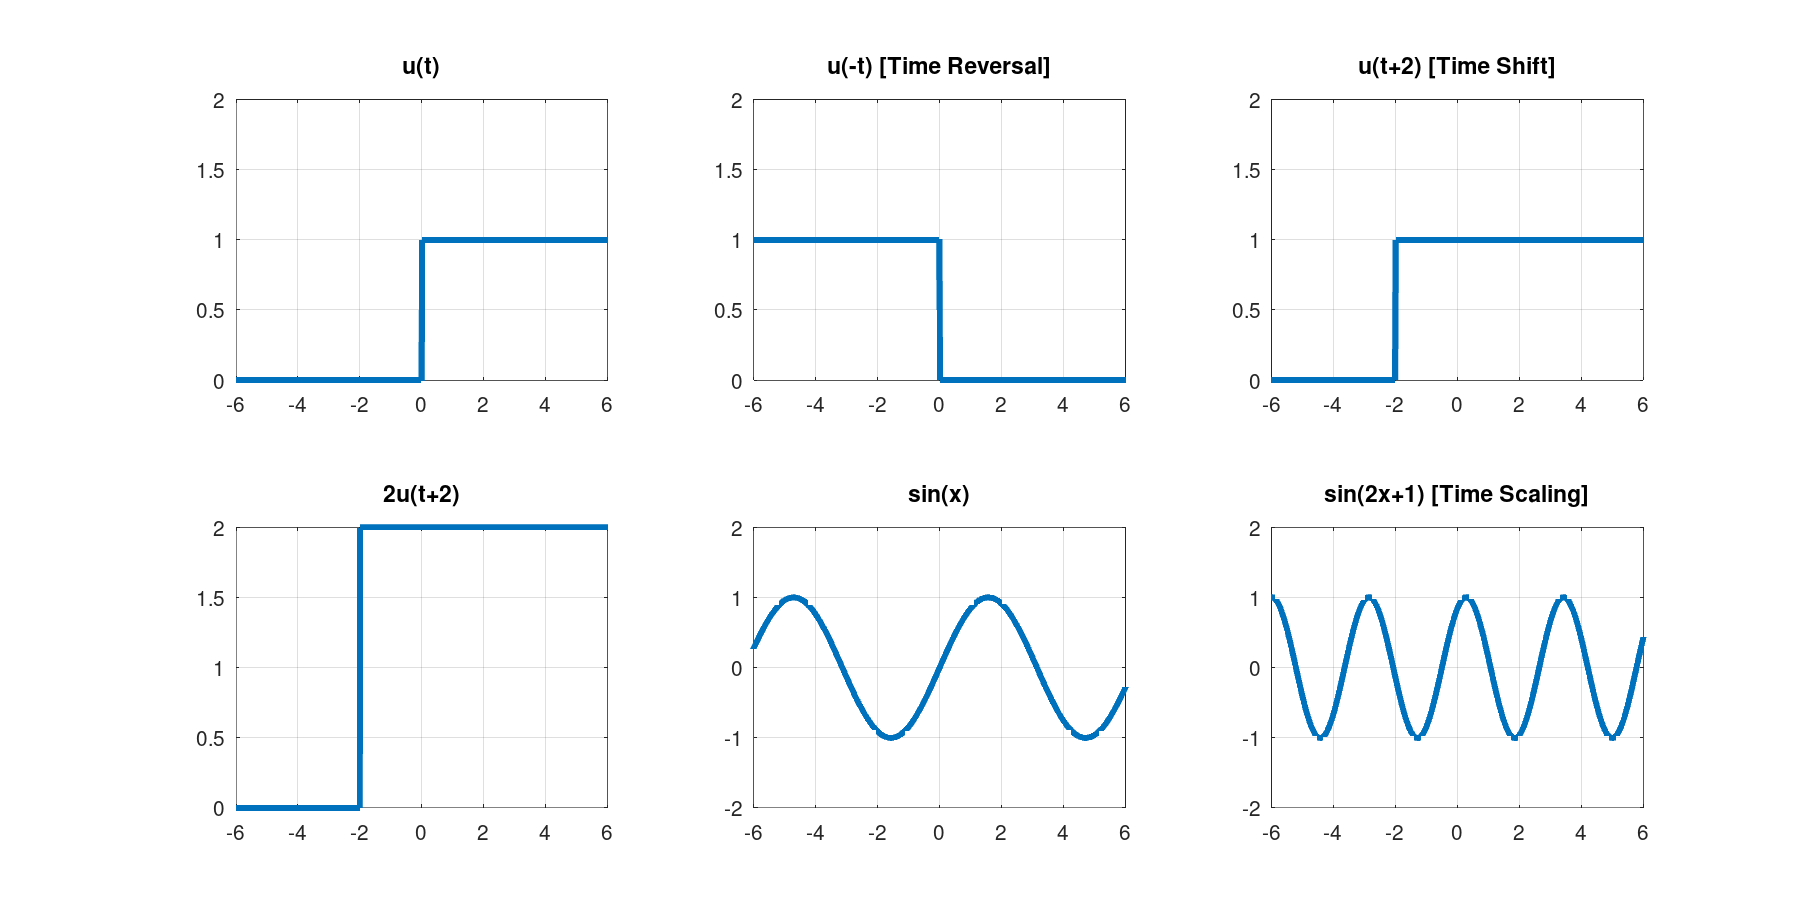
\includegraphics[width=0.8\linewidth]{images/transformations}

		\label{fig:transformations}
	\end{figure}
	
	When transforming a signal, we usually start with any time shifts. Then we apply other transformations such as a time reversal, or time scaling. 
	
	\begin{mdframed}
		\textbf{Ex. } Plot $\cos(-t/2 + 1)$
		
		We take it in 4 steps:
		
		\centering
		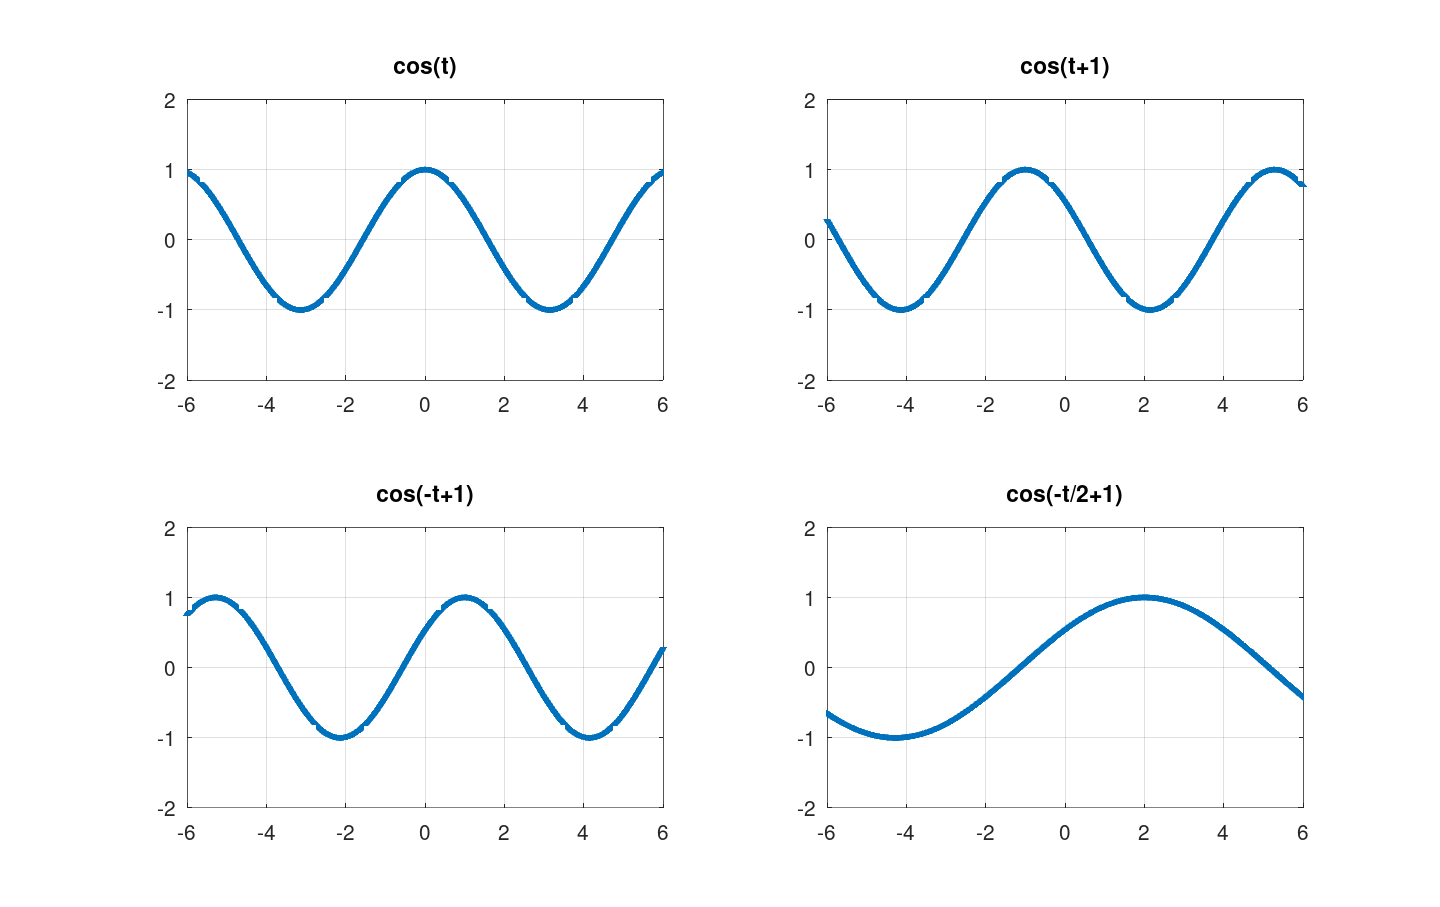
\includegraphics[width=0.8\linewidth]{images/ex1}
	\end{mdframed}
	
	\subsection{Periodicity}
	A signal is called periodic if:
	\begin{align}
		x(t) = x(t+T) \text{  } \forall \text{ }t\label{eq:1}
	\end{align}
	We call the fundamental period $T_0$ the smallest \textit{positive} value of $T$ for which Equation \ref{eq:1} holds.
	
	We have the same idea in discrete time except we change $t$ for $n$, and $T$ for $N$.
	\begin{align}
		x[n] = x[n+N] \text{  } \forall \text{ }n\label{eq:2}
	\end{align}
	
	Note that any complex exponential in the form of $e^{j\omega_0 t}$ is periodic with period $T = \frac{2\pi}{\omega_0}$.
	
	\begin{mdframed}
		\textbf{Ex.} Find the period of $x[n]$.
		\begin{align*}
			x[n] = e^{j(\frac{2\pi}{3})n} + e^{j(\frac{3\pi}{4})n}
		\end{align*}
		I need to find both periods, and find the greatest common multiple. 
		
		Note that since I am in discrete time, the period must be an integer. 
		\begin{align*}
			T_1 &= \frac{2\pi}{\frac{2\pi}{3}} = 3\\
			T_2 &= \frac{2\pi}{\frac{3\pi}{4}} = \frac{8}{3} = 8 \text{ since } \frac{8}{3} \notin \mathbb {Z}\\
			T &= LCM(3,8) = 24
		\end{align*}
	\end{mdframed}
	
	\subsection{Even and Odd Functions}
	We call a signal Even if it satisfies Equation \ref{eq:3} or Odd if it satisfies Equation \ref{eq:4}.
	\begin{align}
		x(t) = x(-t) \label{eq:3}\\
		x(t) = -x(-t) \label{eq:4}
	\end{align}
	We can construct any signal by using its even and odd portions. 
	\begin{align}
		x(t) = Ev\{x(t)\} + Od\{x(t)\} = \frac{1}{2}(x(t) + x(-t)) + \frac{1}{2} (x(t) - x(-t)) \label{eq:5}
	\end{align}
	
	\subsection{Unit Impulse and Unit Step}
	These are two very useful functions as defined below.
	\begin{figure}[!h]
		\centering
		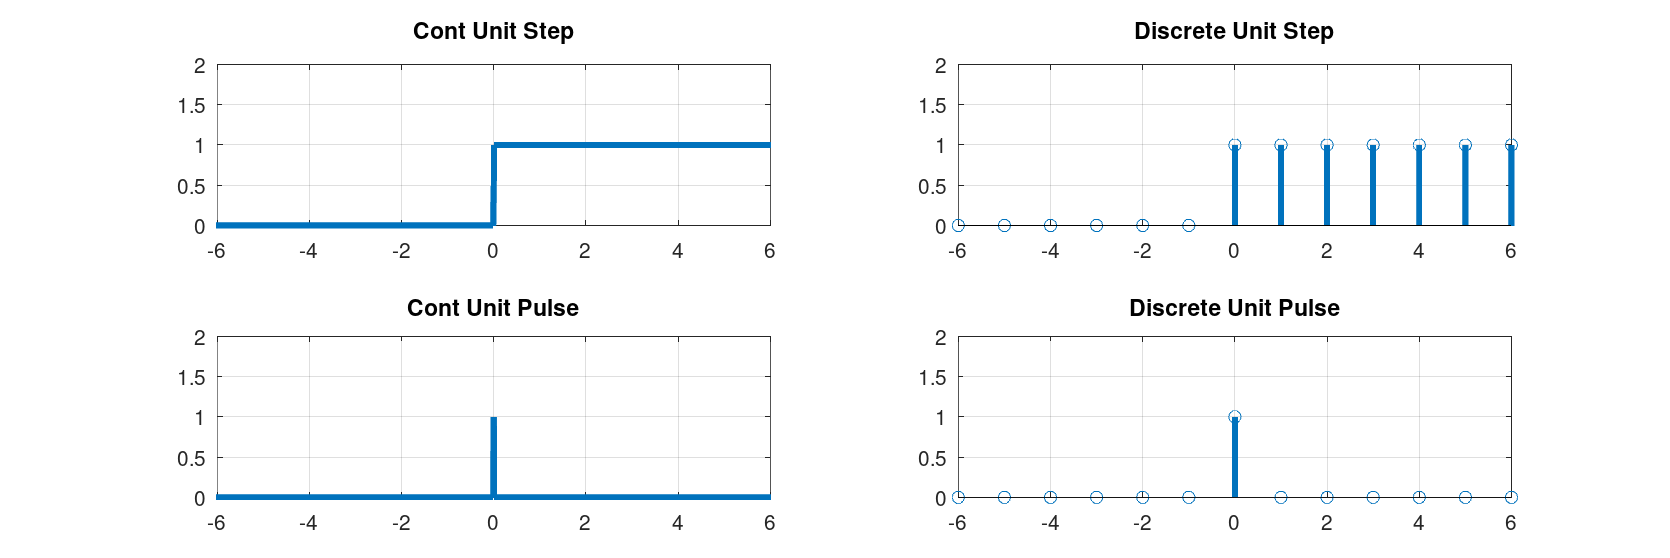
\includegraphics[width=0.9\linewidth]{images/unit step and impulse}
		
		\label{fig:unit}
	\end{figure}
	The unit step is 0 when x is negative, and 1 when positive or 0. The impulse is 1 only when x is 0.
	
	\subsection{System Properties}
	
	\subsubsection{Memory}
	A system is memoryless if the output is only dependant on the input at the same time. 
	
	So basically we do not see any time shifts such as $t-1$ or $t+1$.
	
	\subsubsection{Invertibility}
	A system is invertible if distinct inputs lead to distinct outputs. 
	
	\subsubsection{Causality}
	A system is causal if the output at any time depends only on input values of present and in the past. It does not depend on any future values. 
	
	This is also referred to as being nonanticipative.
	
	Note that all memoryless systems are causal.
	\begin{mdframed}
		\textbf{Ex.}
	\end{mdframed}
	
	\subsubsection{Stability}
	A system is stable if when inputs are bounded, the outputs are always bounded. So:
	\begin{align}
		|x(t)| < \infty \implies |y(t)| < \infty 
	\end{align}
	Assuming $x(t)$ is input, and $y(t)$ is output.
	
	\subsubsection{Time Invariance}
	A system is time invariant if a time shift in the input results in an identical time shift in the output. 
	
	\begin{mdframed}
		\textbf{Ex.}
	\end{mdframed}
	
	\subsubsection{Linearity}
	A system is linear if Equation \ref{eq:6} is satisfied.
	\begin{align}
		ax_1 (t) + bx_2 (t) \to ay_1 (t) + by_2(t)\label{eq:6}
	\end{align}
	
	\begin{mdframed}
		\textbf{Ex. }
	\end{mdframed}
	
	\section{LTI Systems}
	
	\subsection{Convolution in Discrete Time}
	
	\subsection{Convolution in Continuous Time}
	
	\subsection{Differential and Difference Equations}
	
	\section{Fourier Series}
	
	\subsection{Properties of Continuous Fourier Series}
	
	\subsubsection{Linearity}
	
	\subsubsection{Time Shifting}
	
	\subsubsection{Time Reversal}
	
	\subsubsection{Time Scaling}
	
	\subsubsection{Multiplication}
	
	\subsubsection{Conjugate}
	
	\subsubsection{Parseval's Relation}
	
	\subsection{Properties of Discrete Fourier Series}
	
	% MIDTERM MATERIAL ENDS HERE
	\section{Fourier Transformations}
	
	\section{Discrete Time Fourier Transformation}
	
	\section{Filters}
	
	\section{Bode Plot}
	
	\section{Sampling}
	
	\section{Laplace Transformations}
	
	
\end{document}